\section{Regelmäßiges Ausrichten der Wände (Janneke)}

Da das verspätete Aktualisieren des Referenzscans, um drift des Scans über die Zeit abzumildern, nicht ganz den gewünschten Effekt hatte und eher zu mehr Problemen geführt hat haben wir versucht das Problem anders zu lösen. Bei den Tests fällt auf das der Drift der Rotation ein größeres Problem zu sein scheint, als der Translations-drift. Da wir nur ganz am Anfang den initialen Scan auf die Hauptachsen alignen und dann darauf vertrauen, dass alle weiteren Scans durch die Rotationskorrektur richtig ausgerichtet werden liegt es nahe diesen Schritt auch in der Schleife ab und zu durchzuführen. Dies sollte den Drift über die Zeit gut kompensieren können.

Hierbei ist es jedoch wichtig, das Maximum das im Histogramm gefunden wird auf die richtige Achse zu mappen, da je nach Position und Orientierund unterschiedliche Wände im Histogramm besonders stakt erkennbar sind. Hierfür nehmen wir an, das wir gerade Wände, bzw. Linien haben, die 90 Grad aufeinander stehen. Da das Verfahren sowieso auf dieser Annahme beruht schränken wir es also nicht weiter ein. Bei einem Histogramm das auf einem auf die Hauptachsen ausgerichteten Scan berechnet wurde sollen die Peaks nun also auf 0, $\frac{\pi}{2}$, $\pi$, $\frac{3\pi}{2}$ oder $2\pi$ liegen. Wir berechnen nun also die Rotation die das Maximum im Winkelhistogramm auf einen dieser Werte schiebt und wenden diese zusätzlich auf den Scan an, bevor wir diesen in die Karte eintragen. Die Rotation muss natürlich auch auf den globalen Rotationsoffset drauf gerechnet werden, damit spätere Scans auf diesen neuen Scan ausgerichtet werden.

Abbildung~\ref{fig:mitAchsenAlign_1min}-\ref{fig:ohneAchsenAlign_10min} stellen unser Verfahren mit und ohne Ausrichtungsupdate zu unterschiedlichen Fahrzeiten gegenüber. Während die Karten bei einer Fahrzeit von einer Minute noch recht ähnlich aussehen ist bei einer Fahrzeit von 4 Minuten schon gut zu erkennen, das die Karte mit Ausrichtungsupdate (Abbildung~\ref{fig:mitAchsenAlign_4min}) weniger dicke Wände hat als die Karte ohne Ausrichtungsupdate (Abbildung~\ref{fig:ohneAchsenAlign_4min}). Des weiteren ist gut zu erkennen, dass sich die Karten mit Ausrichtungsupdate zwischen einer Fahrzeit von 7 (Abbildung~\ref{fig:mitAchsenAlign_7min}) und 10 (Abbildung~\ref{fig:mitAchsenAlign_10min}) Minuten kaum verändern, während bei den Karten ohne Ausrichtungsupdate erkennbar ist, dass sich die Karte immer weiter verschlechtert (Abbildung~\ref{fig:ohneAchsenAlign_7min} \& \ref{fig:ohneAchsenAlign_10min})  

Die neue Ausrichtung der Scans soll nun aber nicht in jedem Schritt passieren, sondern nur über die Zeit den Drift verhindern. Daher haben wir verschiedene Schrittgrößen angefangen bei jedem 10. Karten-update ausprobiert. Dabei haben wir festgestellt, dass ein Ausrichtungsupdate alle 5 Karten-updates ein guter Wert ist.

\begin{figure}
	\centering
	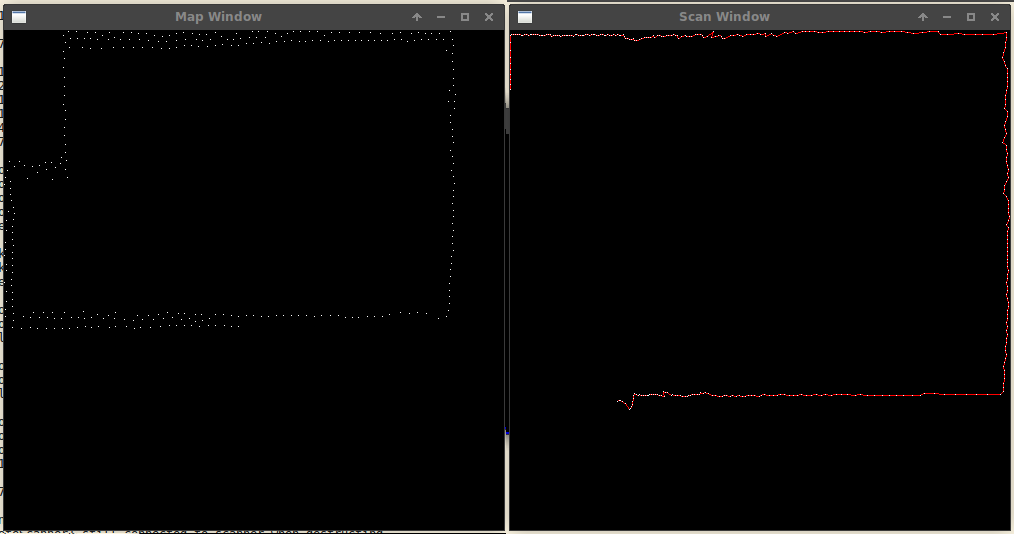
\includegraphics[width=14cm]{mitAchsenAlign_1min_2}
	\caption{Karte mit Ausrichtungsupdate alle 10 Karten-update Schritte, 1min Fahrzeit\newline}
	\label{fig:mitAchsenAlign_1min}
	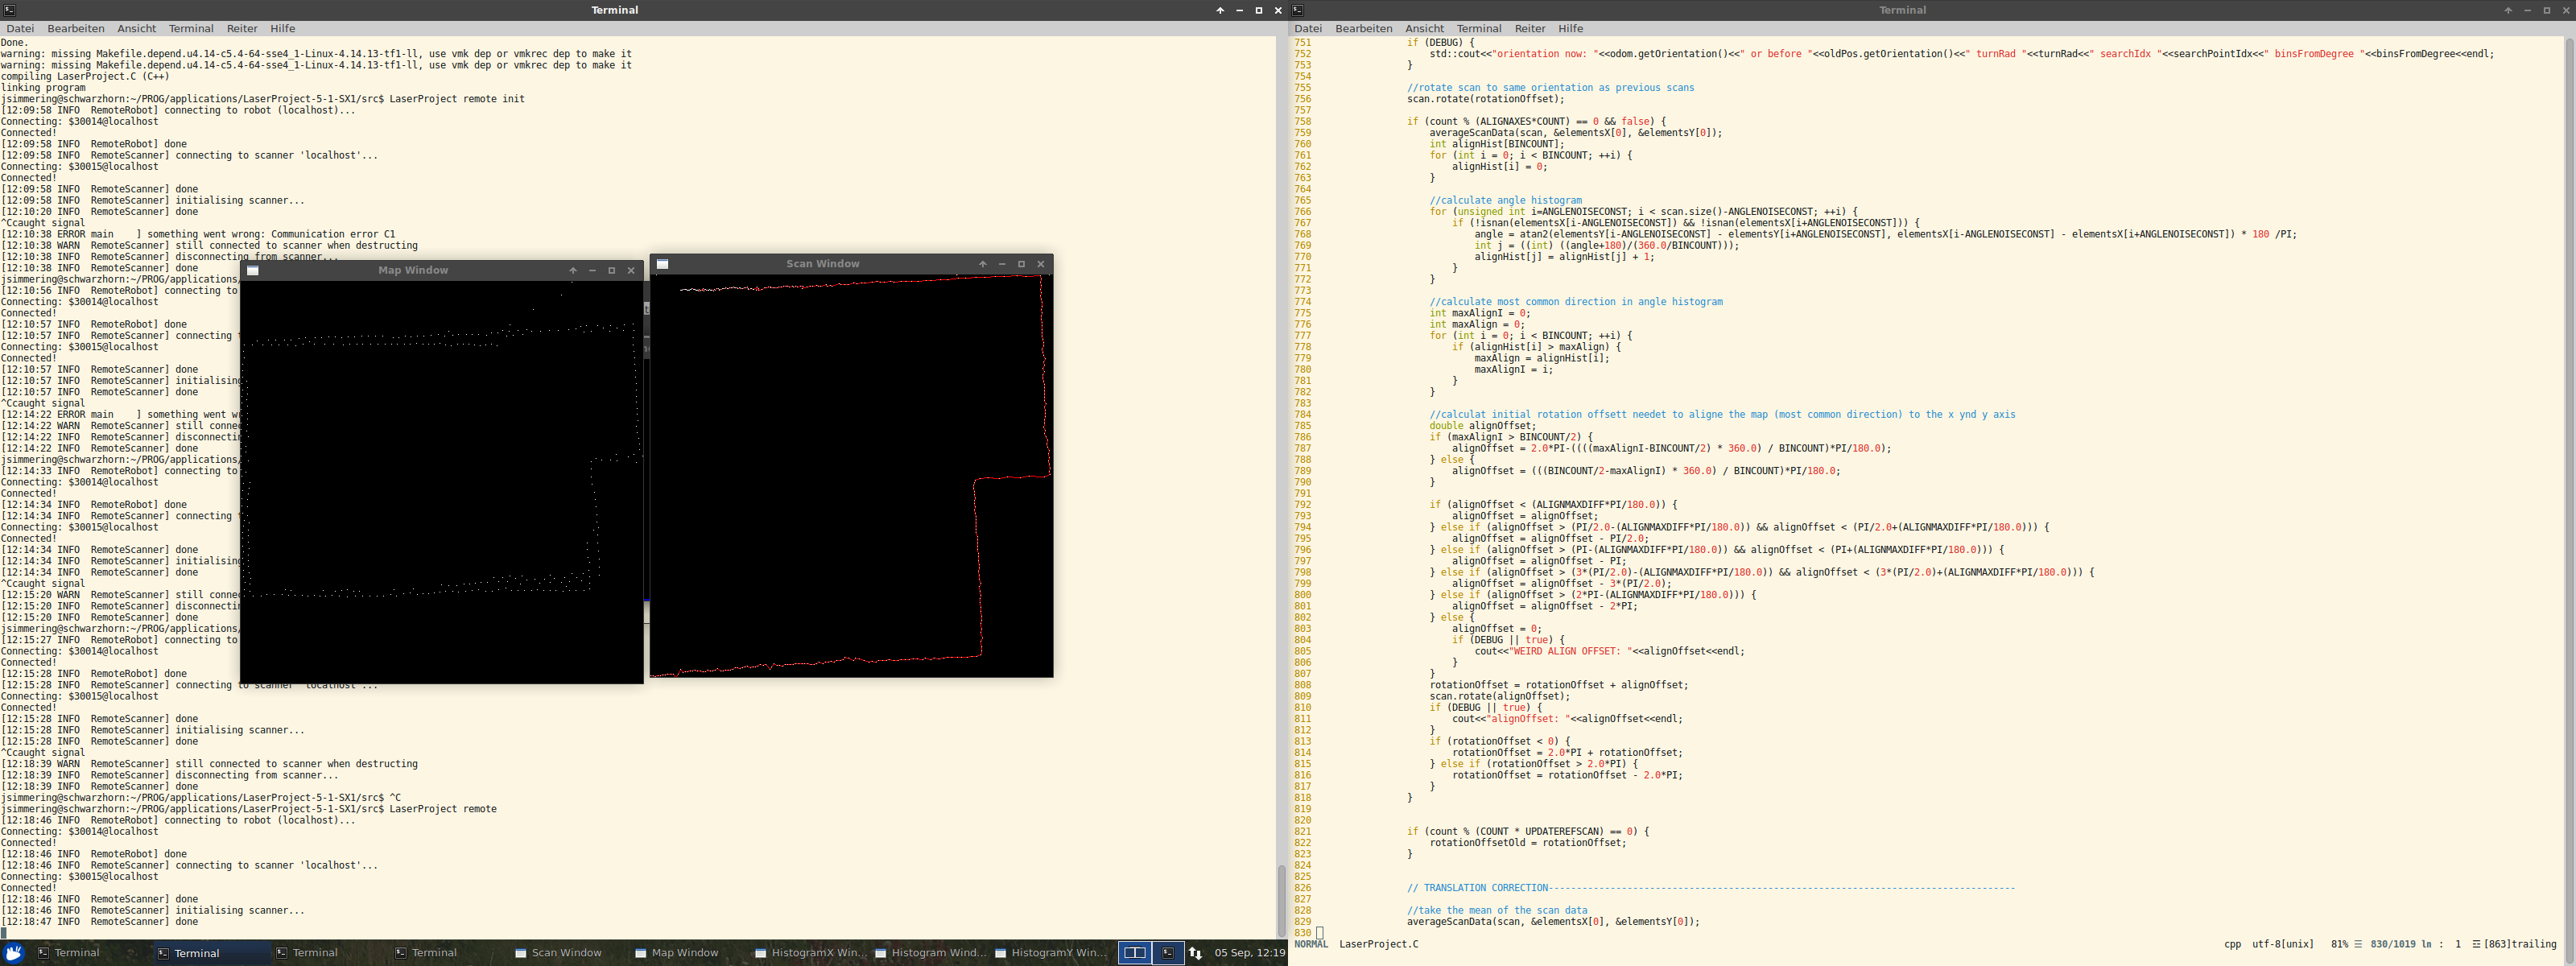
\includegraphics[width=14cm]{ohneAchsenAlign_1min_3}
	\caption{Karte ohne Ausrichtungsupdates, 1min Fahrzeit\newline}
	\label{fig:ohneAchsenAlign_1min}
\end{figure}

\begin{figure}
	\centering
	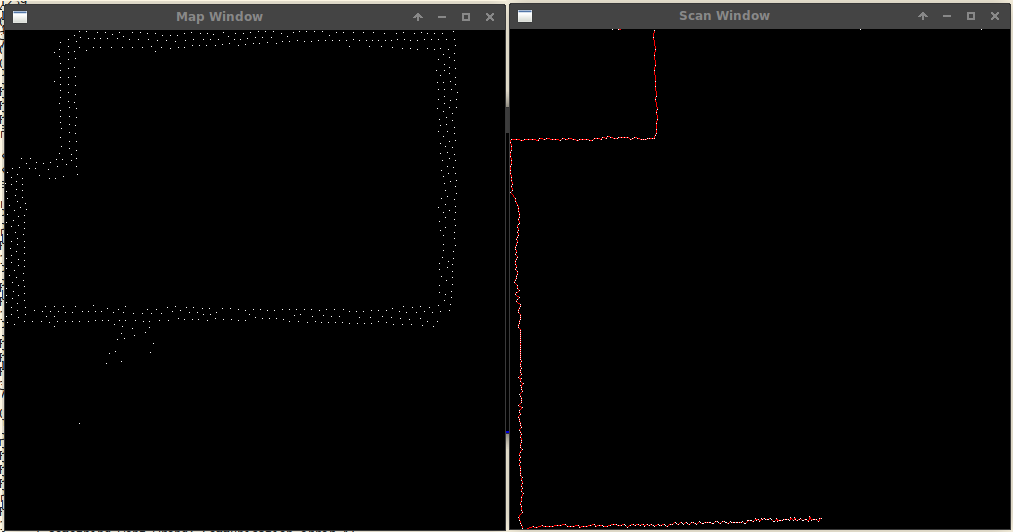
\includegraphics[width=14cm]{mitAchsenAlign_4min_2}
	\caption{Karte mit Ausrichtungsupdate alle 10 Karten-update Schritte, 4min Fahrzeit\newline}
	\label{fig:mitAchsenAlign_4min}
	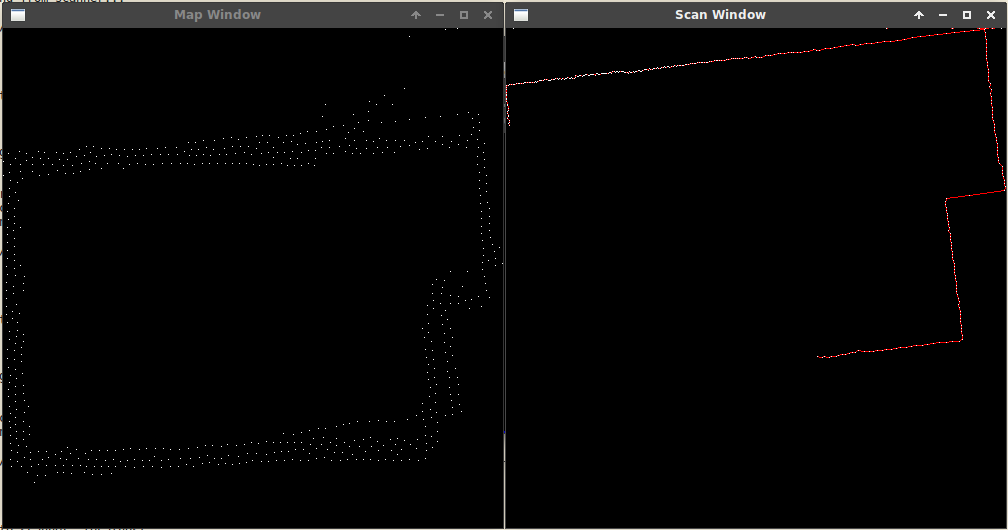
\includegraphics[width=14cm]{ohneAchsenAlign_4min_3}
	\caption{Karte ohne Ausrichtungsupdates, 4min Fahrzeit\newline}
	\label{fig:ohneAchsenAlign_4min}
\end{figure}

\begin{figure}
	\centering
	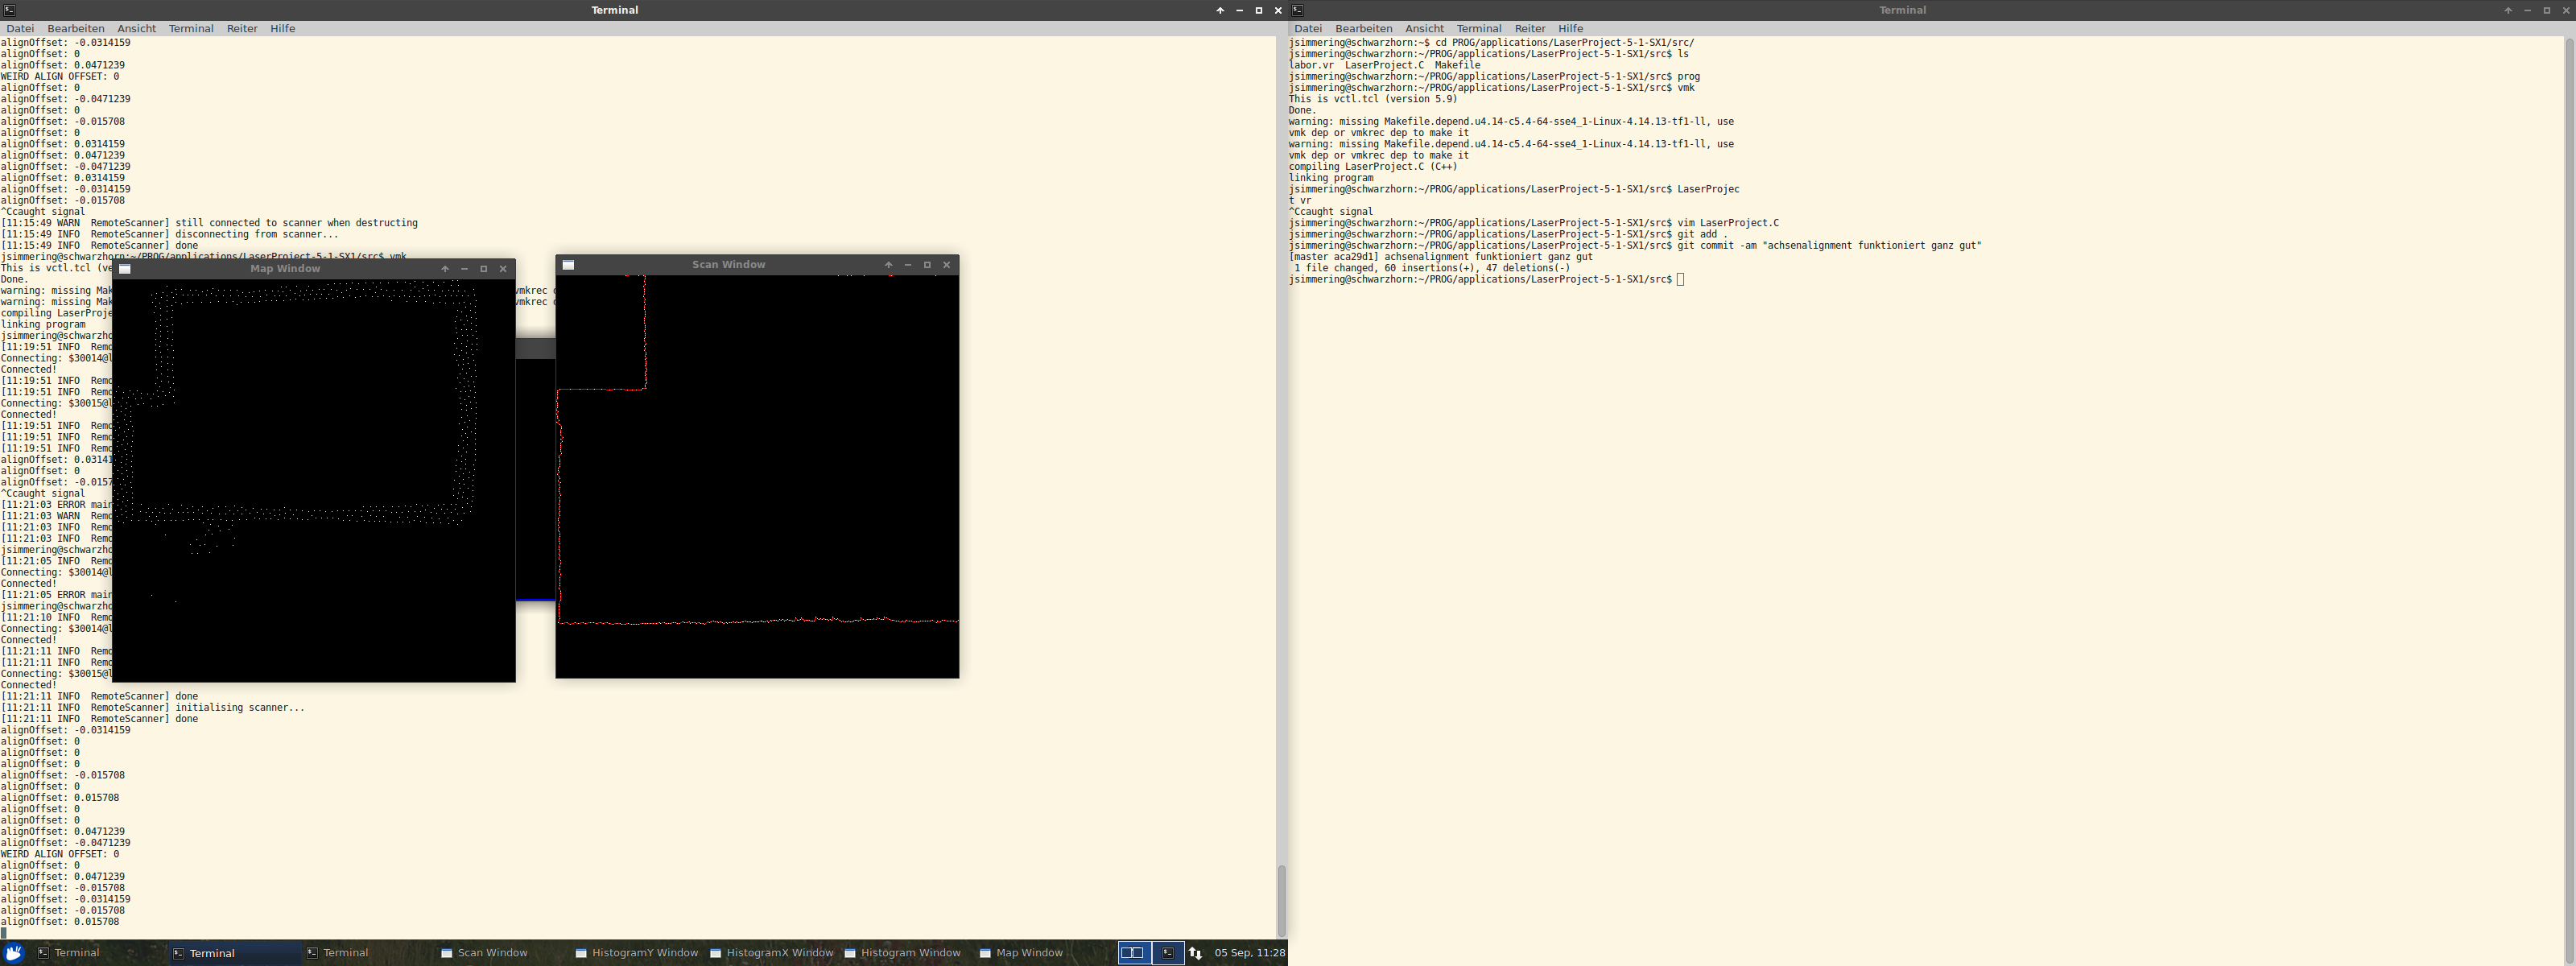
\includegraphics[width=14cm]{mitAchsenAlign_7min_2}
	\caption{Karte mit Ausrichtungsupdate alle 10 Karten-update Schritte, 7min Fahrzeit\newline}
	\label{fig:mitAchsenAlign_7min}
	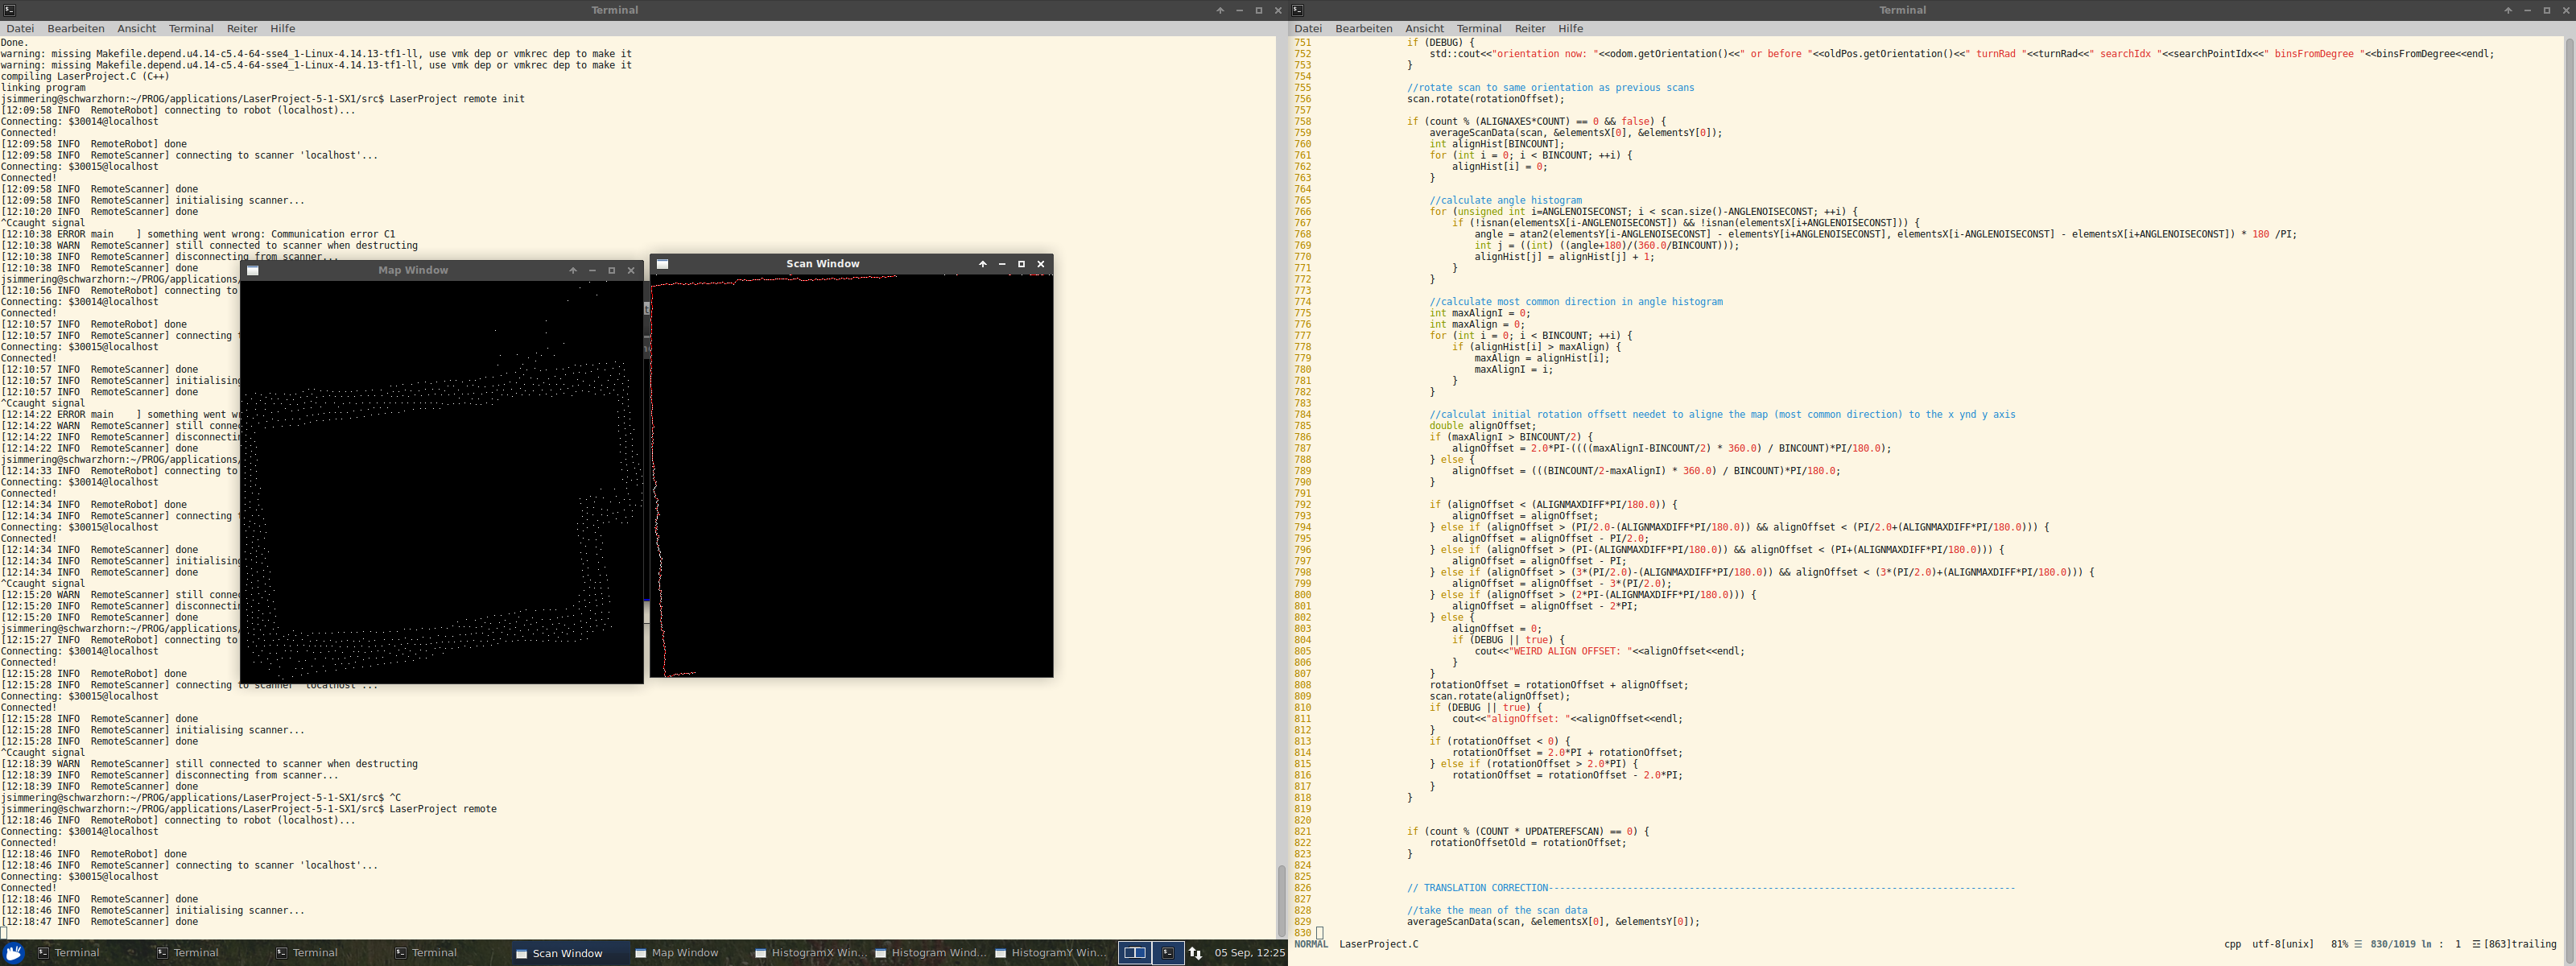
\includegraphics[width=14cm]{ohneAchsenAlign_7min_3}
	\caption{Karte ohne Ausrichtungsupdates, 7min Fahrzeit\newline}
	\label{fig:ohneAchsenAlign_7min}
\end{figure}

\begin{figure}
	\centering
	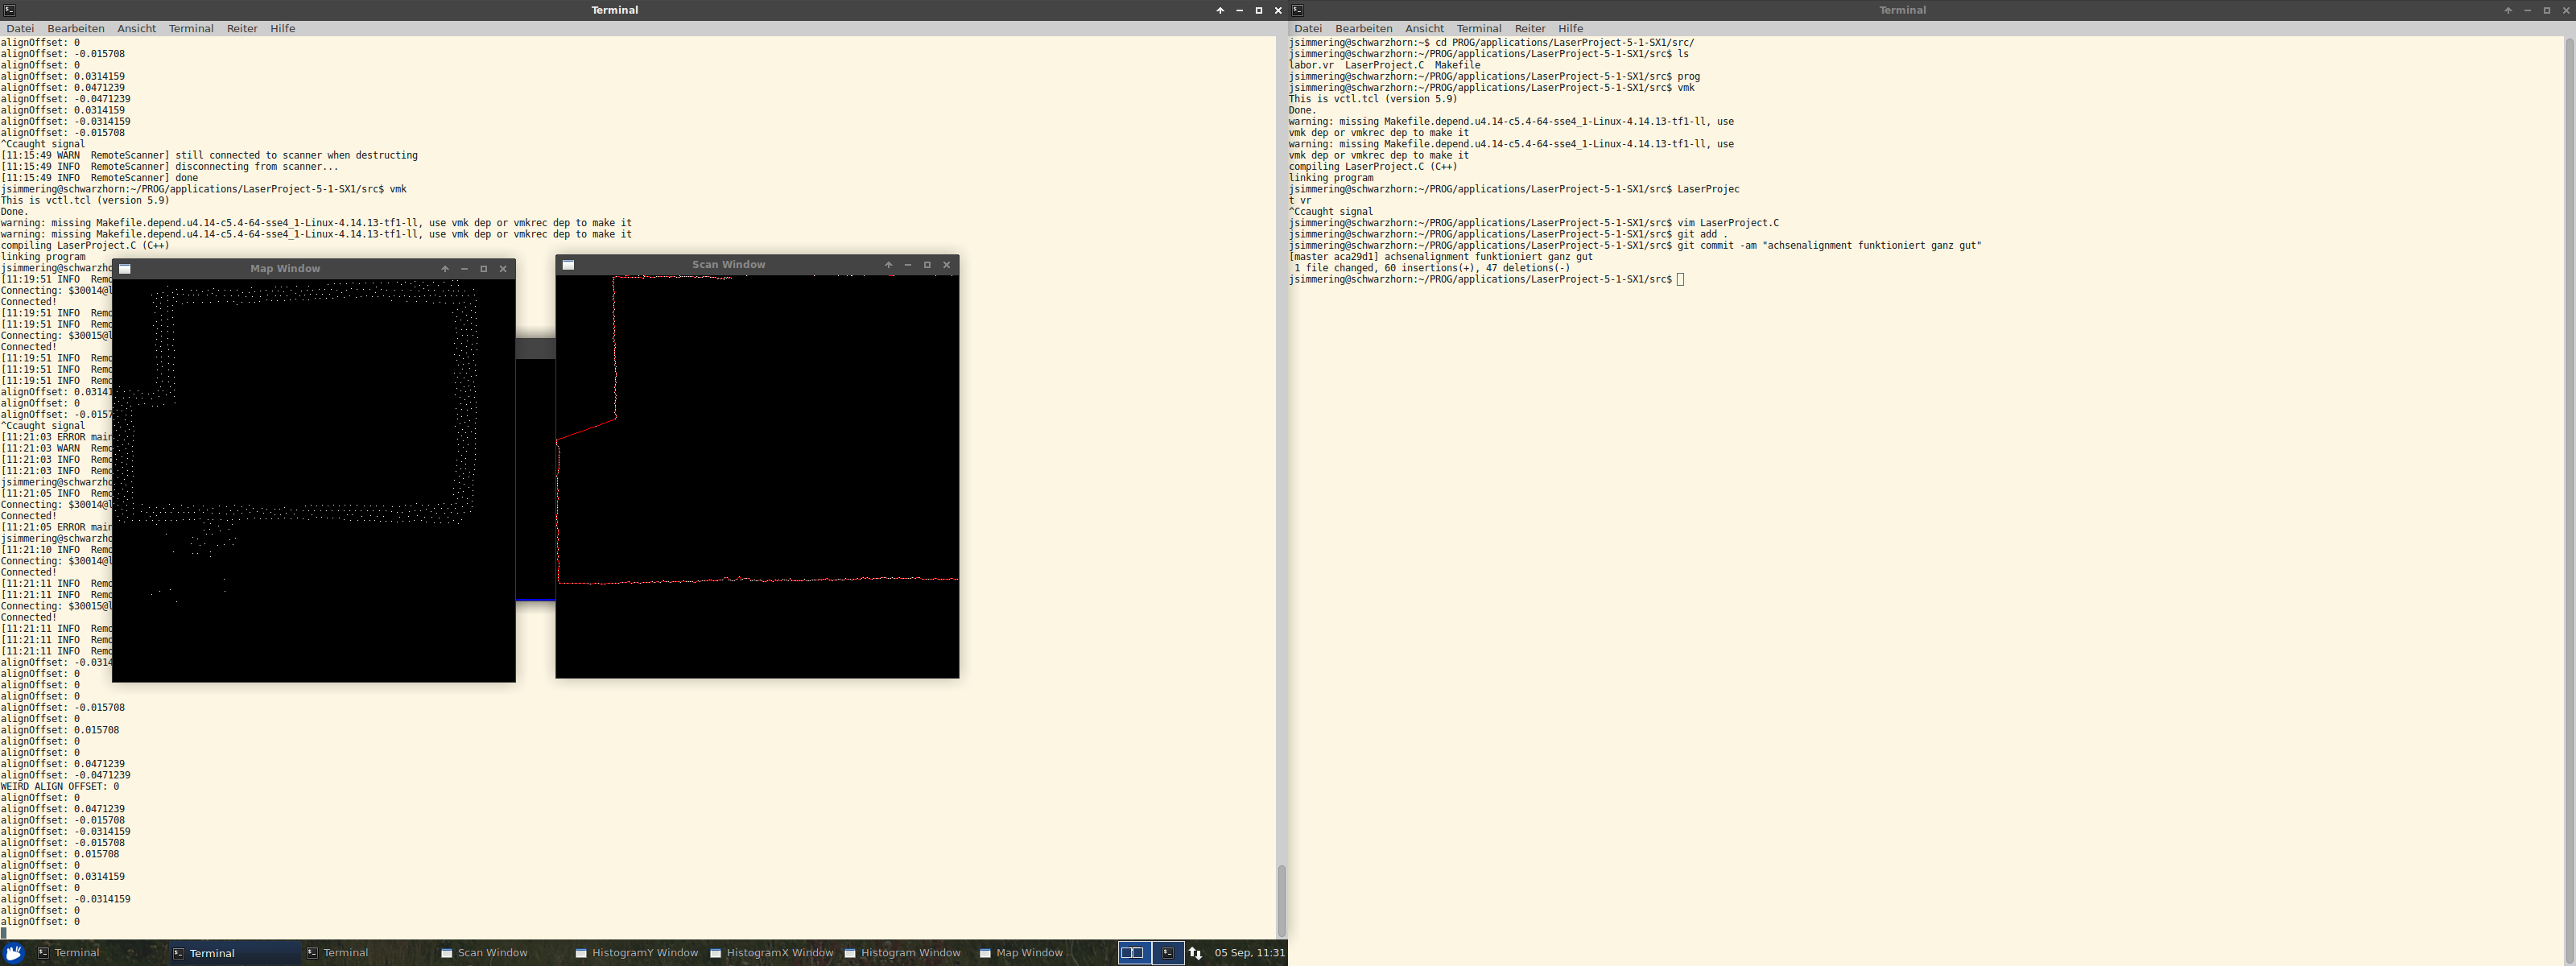
\includegraphics[width=14cm]{mitAchsenAlign_10min_2}
	\caption{Karte mit Ausrichtungsupdate alle 10 Karten-update Schritte, 10min Fahrzeit\newline}
	\label{fig:mitAchsenAlign_10min}
	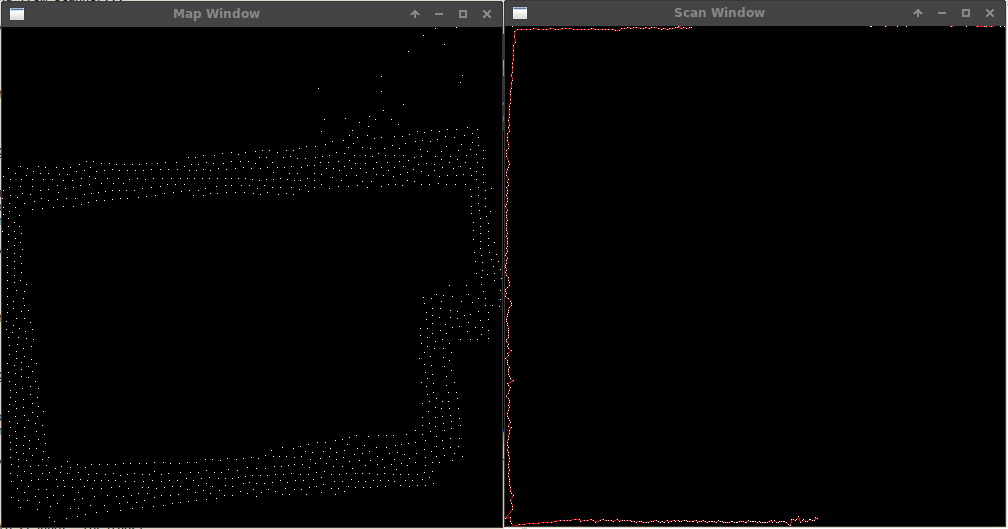
\includegraphics[width=14cm]{ohneAchsenAlign_10min_3}
	\caption{Karte ohne Ausrichtungsupdates, 10min Fahrzeit\newline}
	\label{fig:ohneAchsenAlign_10min}
\end{figure}